\documentclass[conference]{IEEEtran}
\IEEEoverridecommandlockouts
\usepackage{cite}
\usepackage{amsmath,amssymb}
\usepackage{graphicx}
\usepackage{booktabs}
\usepackage{multirow}
\usepackage{xcolor}
\usepackage{tikz}
\usetikzlibrary{positioning,arrows.meta,fit}
\usepackage[hidelinks]{hyperref}
\newcommand{\succNav}{100}
\newcommand{\ttgNav}{43}
\newcommand{\withinNav}{1.46}
\newcommand{\burdenNav}{9.5}
\newcommand{\rateNav}{12.7}
\newcommand{\hlNav}{0.81}
\newcommand{\speedNav}{0.35}
\newcommand{\stopsNav}{4.8}
\newcommand{\succBlind}{100}
\newcommand{\ttgBlind}{38}
\newcommand{\withinBlind}{1.52}
\newcommand{\burdenBlind}{8.4}
\newcommand{\rateBlind}{13.0}
\newcommand{\hlBlind}{0.80}
\newcommand{\speedBlind}{0.39}
\newcommand{\stopsBlind}{3.3}
\newcommand{\succCV}{100}
\newcommand{\ttgCV}{48}
\newcommand{\withinCV}{1.56}
\newcommand{\burdenCV}{9.7}
\newcommand{\rateCV}{11.6}
\newcommand{\hlCV}{0.78}
\newcommand{\speedCV}{0.33}
\newcommand{\stopsCV}{5.0}
\newcommand{\succLSTM}{100}
\newcommand{\ttgLSTM}{50}
\newcommand{\withinLSTM}{1.57}
\newcommand{\burdenLSTM}{9.3}
\newcommand{\rateLSTM}{10.8}
\newcommand{\hlLSTM}{0.75}
\newcommand{\speedLSTM}{0.32}
\newcommand{\stopsLSTM}{5.3}
\newcommand{\succSocial}{97}
\newcommand{\ttgSocial}{58}
\newcommand{\withinSocial}{2.39}
\newcommand{\burdenSocial}{12.5}
\newcommand{\rateSocial}{11.9}
\newcommand{\hlSocial}{0.79}
\newcommand{\speedSocial}{0.28}
\newcommand{\stopsSocial}{6.9}
\newcommand{\succBCa}{78}
\newcommand{\ttgBCa}{97}
\newcommand{\withinBCa}{3.16}
\newcommand{\burdenBCa}{17.6}
\newcommand{\rateBCa}{10.3}
\newcommand{\hlBCa}{0.76}
\newcommand{\speedBCa}{0.16}
\newcommand{\stopsBCa}{5.6}
\newcommand{\succBCb}{88}
\newcommand{\ttgBCb}{94}
\newcommand{\withinBCb}{2.76}
\newcommand{\burdenBCb}{16.8}
\newcommand{\rateBCb}{11.4}
\newcommand{\hlBCb}{0.75}
\newcommand{\speedBCb}{0.17}
\newcommand{\stopsBCb}{6.6}
\newcommand{\adeCV}{1.258}
\newcommand{\fdeCV}{2.845}
\newcommand{\adenearCV}{1.158}
\newcommand{\adeEgo}{1.065}
\newcommand{\fdeEgo}{2.322}
\newcommand{\adenearEgo}{1.063}
\newcommand{\adeSoc}{0.946}
\newcommand{\fdeSoc}{1.944}
\newcommand{\adenearSoc}{0.948}
\newcommand{\adeRob}{0.952}
\newcommand{\fdeRob}{1.933}
\newcommand{\adenearRob}{0.935}
\newcommand{\dvelKeep}{0.059}
\newcommand{\dspdKeep}{0.037}
\newcommand{\dyieldKeep}{83}
\newcommand{\dvelGoal}{0.121}
\newcommand{\dspdGoal}{0.095}
\newcommand{\dyieldGoal}{12}
\newcommand{\dvelBlind}{0.054}
\newcommand{\dspdBlind}{0.038}
\newcommand{\dyieldBlind}{88}
\newcommand{\dvelSocial}{0.054}
\newcommand{\dspdSocial}{0.039}
\newcommand{\dyieldSocial}{88}
\newcommand{\dvelNocopy}{0.074}
\newcommand{\dspdNocopy}{0.045}
\newcommand{\dyieldNocopy}{85}
\newcommand{\dvelPeople}{0.131}
\newcommand{\dspdPeople}{0.102}
\newcommand{\dyieldPeople}{10}
\newcommand{\humSpeed}{0.24}
\newcommand{\humStops}{3.2}
\newcommand{\humTTC}{2.0}
\newcommand{\humMinDist}{0.82}
\newcommand{\humMinutes}{32}
\newcommand{\humPass}{1.42}


\begin{document}

\title{Learned Pedestrian Prediction for Nav2 in Data-Calibrated Reactive Crowds, Measured against a Human-Driven Robot}

\author{\IEEEauthorblockN{Filmon Nezif Abamecha}
\IEEEauthorblockA{Higher Colleges of Technology\\ United Arab Emirates}}

\maketitle

\begin{abstract}
Social navigation methods are usually judged on how close the robot came to people. That number alone misses what makes a robot unpleasant to walk next to: jerky stops, sudden turns, and pushing people off their path. We ask whether learning from real human--robot interaction data makes a standard ROS~2/Nav2 robot move through crowds more like a human-driven robot. Using the TH\"OR-MAGNI dataset, in which people walk around a teleoperated robot, we (i) train an LSTM pedestrian predictor that lowers displacement error by 25\% against constant velocity, (ii) feed its forecasts to Nav2 through a costmap layer, (iii) replay recorded people in Gazebo who react to the robot with a model calibrated to the data, and (iv) clone the human operator's speed choices. Over 32 paired runs per set-up with a robot of the dataset robot's size, learned prediction lowered the rate at which the robot displaced people by 15\% (95\% CI 4--26\%) and gave the motion closest to the human driver's, at the cost of a 14\% longer trip, so total displacement was unchanged. Behaviours that slowed the robot down, a rule-based yielding policy and the cloned driver, added total displacement because the robot stayed among people for longer. The cloned driver failed in closed loop through two known shortcuts of behaviour cloning, and its people-only variant showed that the operator's speed is barely explained by the people around it in this dataset. Code, data processing, recordings and all 224 episodes are released.
\end{abstract}

\begin{IEEEkeywords}
social navigation, trajectory prediction, Nav2, behaviour cloning, human-robot interaction
\end{IEEEkeywords}

\section{Introduction}
A robot that shares a corridor or a lab with people needs more than collision avoidance. People notice when a robot brakes for no reason, swerves late, or forces them to step aside~\cite{kruse2013survey,mavrogiannis2023core}. Standard planners such as Nav2~\cite{macenski2020nav2} treat people as obstacles at their current position. A common remedy is to forecast where people will walk and plan around the forecast~\cite{rudenko2020survey,trautman2010unfreezing}. Whether such forecasts help is usually tested with proximity metrics in simulated crowds whose people either ignore the robot or follow hand-tuned social forces~\cite{helbing1995social,biswas2022socnavbench}.

Recent evaluation guidelines~\cite{francis2023principles} argue for metrics that capture comfort and legibility, and for comparisons with human behaviour. We follow that advice with one dataset that supports all three parts of the question. TH\"OR-MAGNI~\cite{schreiter2024thor} records people with motion capture while a human operator drives a robot (DARKO) among them. The people give us training data for prediction and evidence of how people react to a robot. The operator gives us a human reference for how a robot \emph{should} move.

Our aim is to make a ROS~2/Nav2 robot move through real recorded crowds more like a human-driven robot: smoothly, legibly, and without pushing people aside. Our contributions are:
\begin{itemize}
\item An open ROS~2 Jazzy pipeline that turns TH\"OR-MAGNI recordings into Gazebo scenes, with a cleaning step that raises tracked coverage from about 65\% to 99\%.
\item An LSTM predictor trained on TH\"OR-MAGNI and a Nav2 costmap layer that paints its forecasts.
\item A reactive crowd calibrated to how much real participants kept away from the robot \emph{and} how much extra effort they spent doing so.
\item An evaluation with a burden metric (how far people are pushed off their recorded paths) and a human-likeness distance to the human driver, comparing six set-ups in 32 paired runs each, including a cloned human driver and a negative result on why it failed.
\end{itemize}

\section{Related Work}
\textbf{Prediction for navigation.} Learned trajectory predictors model how people interact~\cite{alahi2016social,rudenko2020survey}, but a constant-velocity model is a strong baseline~\cite{scholler2020cv}. Coupling prediction with planning can avoid the ``freezing robot'' problem~\cite{trautman2010unfreezing}, and recent work couples learned forecasts with model predictive control~\cite{samavi2023sicnav}. Reinforcement learning methods learn the policy directly in simulation~\cite{chen2019crowd}, and inverse reinforcement learning recovers cost functions from demonstrations~\cite{kretzschmar2016irl}. We keep Nav2's planner and controller and change only what they see, so the effect of prediction is isolated.

\textbf{Evaluation.} Surveys and guidelines~\cite{mavrogiannis2023core,francis2023principles} note that proximity and success rates do not capture comfort, and recommend path irregularity, jerk, and comparison with human trajectories. SocNavBench~\cite{biswas2022socnavbench} replays real pedestrians who do not react to the robot. We replay real pedestrians but let them react, and we calibrate that reaction to data.

\textbf{Learning from human drivers.} Datasets of human-teleoperated robots such as SCAND~\cite{karnan2022scand} and of humans walking with sensors such as MuSoHu~\cite{nguyen2023musohu} support learning human-like navigation. Behaviour cloning from observation histories is known to fail by copying its own past actions~\cite{wen2020copycat} or by relying on other spurious inputs~\cite{dehaan2019causal,codevilla2019limits}. We observe both failures and report them.

\section{Method}

\begin{figure}[t]
\centering
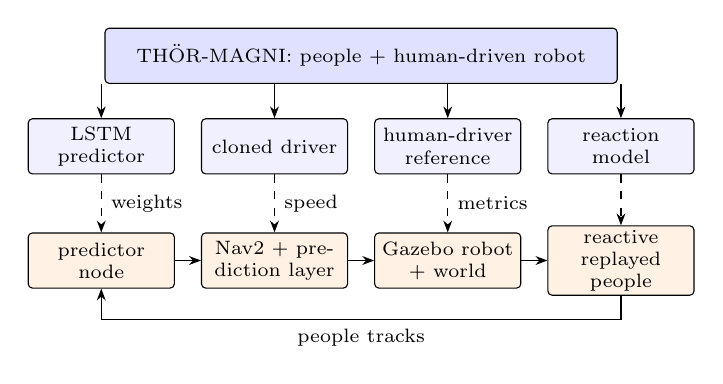
\begin{tikzpicture}[font=\scriptsize, x=2.2cm, y=1cm,
  box/.style={draw, rounded corners=1.5pt, align=center, text width=1.75cm, minimum height=7mm, inner sep=1.5pt},
  off/.style={box, fill=blue!6}, run/.style={box, fill=orange!10}, >={Stealth[length=1.5mm]}]
\node[box, fill=blue!12, text width=6.4cm] (data) at (1.5, 1.15) {TH\"OR-MAGNI: people + human-driven robot};
\node[off] (pred) at (0,0) {LSTM predictor};
\node[off] (bc) at (1,0) {cloned driver};
\node[off] (ref) at (2,0) {human-driver reference};
\node[off] (rea) at (3,0) {reaction model};
\foreach \n in {pred,bc,ref,rea} \draw[->] (data.south -| \n) -- (\n);
\node[run] (pn) at (0,-1.45) {predictor node};
\node[run] (nav) at (1,-1.45) {Nav2 + prediction layer};
\node[run] (gz) at (2,-1.45) {Gazebo robot + world};
\node[run] (ppl) at (3,-1.45) {reactive replayed people};
\draw[->, dashed] (pred) -- node[right]{weights} (pn);
\draw[->, dashed] (bc) -- node[right]{speed} (nav);
\draw[->, dashed] (rea) -- (ppl);
\draw[->, dashed] (ref) -- node[right]{metrics} (gz);
\draw[->] (pn) -- (nav);
\draw[->] (nav) -- (gz);
\draw[->] (gz) -- (ppl);
\draw[->] (ppl.south) -- ++(0,-0.3) -| node[pos=0.25, below]{people tracks} (pn.south);
\end{tikzpicture}
\caption{Offline learning (blue) and the ROS~2 runtime (orange). Every episode is recorded as a rosbag and a video.}
\label{fig:system}
\end{figure}

\subsection{Data and scenes}
We use Scenario~3 of TH\"OR-MAGNI~\cite{schreiter2024thor}: recordings of about 4~min on four days, with up to nine people and the DARKO robot (about $0.90\times0.75$~m) in a $9\times10$~m lab. The motion-capture system often fails to solve a helmet as a rigid body while its markers are visible. When this happens we use the mean of the visible markers (2--8~cm from the solved centroid where both exist), which raises coverage from about 65\% to 99\%. A rolling-median filter and a 2.5~m/s speed gate remove jumps to another helmet, and short gaps are interpolated and flagged.

Each recording becomes a Gazebo Harmonic~\cite{koenig2004gazebo} world built from the dataset's floor map, a Nav2 occupancy map, and a file of people trajectories (Fig.~\ref{fig:scene}). The robot uses Nav2 on ROS~2 Jazzy~\cite{macenski2022ros2} with the NavFn planner and the MPPI controller~\cite{williams2016mppi}, and the DARKO footprint. It sees people with its lidar, as obstacles at their current position. Each scene is a 110~s window, and the robot crosses the room in each direction, giving two paired runs per window.

\begin{figure}[t]
\centering
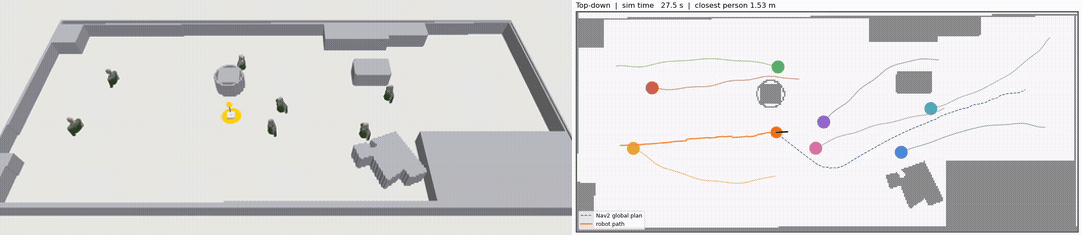
\includegraphics[width=\columnwidth]{figs/scene.png}
\caption{A replayed TH\"OR-MAGNI scene: Gazebo view (left) and top-down view with the Nav2 plan (dashed) and recorded paths (right).}
\label{fig:scene}
\end{figure}

\subsection{Pedestrian predictor}
The predictor observes 3.2~s (8 steps at 2.5~Hz) and forecasts 4.8~s (12 steps) in a frame centred on the person and aligned with their last heading. Variants add the four nearest people and the robot as extra inputs. Each model is a single 128-unit LSTM~\cite{hochreiter1997lstm} with a two-layer fully connected head. Models were trained in MATLAB Online on 36k snippets, split by recording day so that the test day (17~May, 13k snippets) was never seen in training, with three seeds per model. The exported weights run in a NumPy node inside ROS~2, which publishes each person's forecast at 2.5~Hz.

\subsection{Prediction costmap layer}
A C++ Nav2 costmap plugin paints a disc of radius 0.45~m around every forecast point. Point $k$ of the forecast gets cost $w_k \cdot 200$, with $w_k$ falling linearly from 1 to 0.5 over the horizon. The layer runs after inflation in both the global and local costmaps. Forecasts older than 1~s are dropped. All other Nav2 parameters are the stock defaults, so the set-ups differ only in this layer.

\subsection{A reactive crowd calibrated to data}
Recorded people do not react to our robot, which makes a planner look worse than it is, and a robot that ignores people look better than it is. We therefore let each replayed person deviate from their recorded path by an offset $\mathbf{o}$:
\begin{equation}
\ddot{\mathbf{o}} = A\, e^{-(d-R)/B}\,\mathbf{n} - k\,\mathbf{o} - c\,\dot{\mathbf{o}},
\end{equation}
where $d$ is the distance to the robot and $\mathbf{n}$ points away from it. The person is repelled from the robot and pulled back to their path by a damped spring.

A direct fit of this force to TH\"OR-MAGNI accelerations explained none of the variance ($A\approx0$). We therefore calibrate to two statistics. The first is the occupancy ratio: how often people were at a given distance from the real robot, divided by how often they would have been there had the robot driven the same path at a shifted time (a placebo). Real people were almost never within 0.75~m of the robot (Fig.~\ref{fig:reaction}, left). Fitting only this ratio yields people who sidestep by about 1.5~m, with far more extra acceleration than real participants showed. The second statistic is this extra effort: RMS acceleration above the placebo level at each distance. With both, the fit settles on $A=1$, $B=0.7$, $R=0.7$, $k=2$, $c=2.8$. People then match the real effort but not the real occupancy (Fig.~\ref{fig:reaction}). Our reading is that most of the space around the real robot came from its \emph{operator} steering away from people, not from people stepping aside. In our simulation, keeping that space is therefore the robot's job. A half-strength version of the model checks sensitivity.

\begin{figure}[t]
\centering
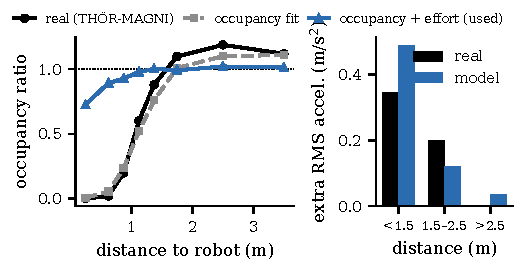
\includegraphics[width=\columnwidth]{figs/reaction.pdf}
\caption{Reaction calibration. Left: how often people were at each distance from the robot relative to a time-shifted placebo. Right: extra RMS acceleration people spent near the robot. Matching both leaves most of the observed clearance to the robot.}
\label{fig:reaction}
\end{figure}

\subsection{Set-ups}
All set-ups use the same Nav2 stack and DARKO footprint:
\begin{itemize}
\item \textbf{Nav2}: stock costmaps; people appear only through the lidar.
\item \textbf{Blind}: Nav2 without obstacle layers, so it ignores people (the collision monitor still stops it before contact). This control tests whether a robot can simply drive straight and let people move.
\item \textbf{CV} / \textbf{LSTM}: Nav2 plus the prediction layer fed by constant-velocity or LSTM forecasts.
\item \textbf{Social}: LSTM plus a rule-based yielding governor that rolls the plan forward, finds the first predicted conflict closer than 0.8~m, and lowers Nav2's speed limit with the time left before it. Its speed and acceleration limits are set from the human driver's 95th percentiles (0.47~m/s, 0.4~m/s$^2$).
\item \textbf{BC}: LSTM plus a cloned human driver that sets the speed limit (Section~\ref{sec:bc}).
\end{itemize}

\subsection{Implementation}
Everything runs headless in a Podman container (ROS~2 Jazzy, Nav2, Gazebo Harmonic) on a laptop with an integrated Intel GPU. Each episode records a rosbag (MCAP) and an MP4 video rendered from the bag, so every number in this paper can be traced to a recording. An episode takes about 1--2~min of wall time, and the final grid of 224 episodes ran overnight. Training ran in MATLAB Online; the exported weights are plain arrays, and a NumPy re-implementation reproduces the MATLAB test metrics, so the robot needs no MATLAB at run time.

\subsection{Metrics}
Besides success, time to goal and time within 0.5~m~\cite{hall1966hidden}, we report two metrics that target the user's concern that closeness alone is not what upsets people.

\textbf{Burden} is the person-seconds during which reactive people were more than 0.2~m off their recorded path. It measures how much the robot made people move. Because slower robots spend longer in the room, we also report burden per minute of driving (the burden rate).

\textbf{Human-likeness distance} compares the robot's motion with that of the human-driven DARKO in ten driving segments of TH\"OR-MAGNI Scenario~3A, where DARKO is teleoperated (\humMinutes~min). For six features (speed, acceleration, jerk, turn rate, speed towards people within 1.5~m, and clearance when passing a person), we take the 1-Wasserstein distance between the pooled robot and human samples, divide it by the human interquartile range, and average. Zero means identical distributions. We also report stop-starts per minute and time with time-to-collision under 2~s. Differences use paired bootstrap 95\% confidence intervals~\cite{efron1993bootstrap} over the 32 scene/direction pairs.

\section{Results}

\subsection{Prediction}
Table~\ref{tab:pred} shows test-day errors. Learning reduced ADE by 25\% and FDE by 32\% against constant velocity, which supports our first hypothesis (a gain of at least 15\%). Most of the gain came from seeing nearby people. Adding the robot as an input improved ADE near the robot by only 1.4\%. This was consistent in three of four test recordings but is about twice the seed-to-seed spread, so it is not clear evidence that people reacted to the robot. Our second hypothesis is therefore not supported. We used the robot-aware model in navigation. Fig.~\ref{fig:predex} shows typical forecasts: the LSTM bends with turns that constant velocity misses, but, as a deterministic model, it averages over sharp changes of direction.

\begin{figure}[t]
\centering
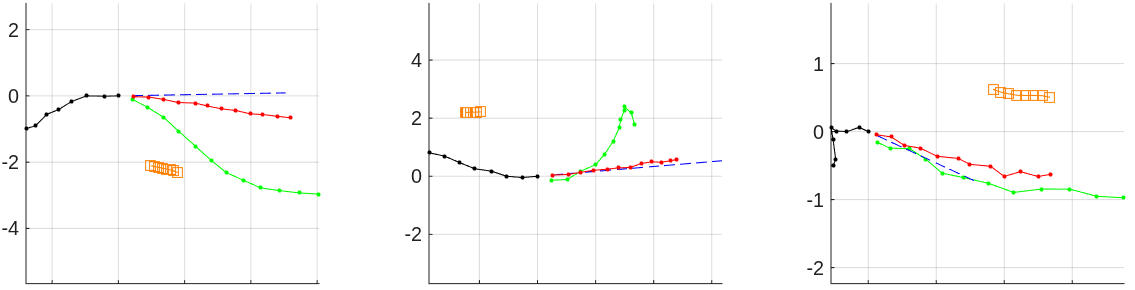
\includegraphics[width=\columnwidth]{figs/pred_examples.png}
\caption{Test-day forecasts (m, person frame): past (black), true future (green), constant velocity (blue dashed), LSTM with people (red), robot (orange squares).}
\label{fig:predex}
\end{figure}

\begin{table}[t]
\centering
\caption{Prediction error on the held-out day (mean of 3 seeds)}
\label{tab:pred}
\begin{tabular}{lccc}
\toprule
Model & ADE (m) & FDE (m) & ADE, robot $<$3~m \\
\midrule
Constant velocity & \adeCV & \fdeCV & \adenearCV \\
LSTM, own motion & \adeEgo & \fdeEgo & \adenearEgo \\
LSTM + 4 nearest people & \textbf{\adeSoc} & \fdeSoc & \adenearSoc \\
LSTM + people + robot & \adeRob & \textbf{\fdeRob} & \textbf{\adenearRob} \\
\bottomrule
\end{tabular}
\end{table}

\subsection{First experiment: a small robot among non-reacting people}
We first ran Nav2, CV, LSTM and Social with a TurtleBot-sized robot (0.22~m radius) among people who replay their recordings without reacting (32 paired runs each). Table~\ref{tab:small} shows that prediction made the robot hesitate. Stop-starts rose by 33\% with CV (95\% CI $[+14, +53]$\%) and by 40\% with LSTM ($[+15, +64]$\%), and both moved \emph{away} from the human driver's motion. Time within 0.5~m fell by 14\% with CV, but the interval included zero. A small robot can slip through gaps that the forecasts close, and people who never step aside punish any hesitation. This set-up is unrealistic in both respects, and it motivated the final experiment: the dataset robot's size and a crowd that reacts as real people did.

\begin{table}[t]
\centering
\caption{Small robot among non-reacting replayed people (32 runs each)}
\label{tab:small}
\setlength{\tabcolsep}{4pt}
\begin{tabular}{lccccc}
\toprule
Set-up & Success & Time to & Within & Stop-starts & Human- \\
 & (\%) & goal (s) & 0.5~m (s) & (/min) & likeness \\
\midrule
Nav2 & 94 & 41 & 2.34 & 4.2 & \textbf{0.80} \\
CV prediction & \textbf{100} & 47 & \textbf{2.01} & 5.8 & 0.84 \\
LSTM prediction & 94 & 50 & 2.16 & 5.8 & 0.87 \\
Social & 97 & 54 & 2.69 & 6.7 & 0.89 \\
\bottomrule
\end{tabular}
\end{table}

\subsection{Navigation in the reactive crowd}
Table~\ref{tab:nav} and Fig.~\ref{fig:results} summarise 224 episodes: 16 test-day scenes, two directions, and seven set-ups, including two versions of the cloned driver.

\begin{table*}[t]
\centering
\caption{Navigation among reactive replayed people (DARKO footprint, 32 paired runs per set-up). Burden: person-seconds people spent more than 0.2~m off their path. Human-likeness: normalised Wasserstein distance to the human-driven robot (lower is more human-like). Human driver: speed \humSpeed~m/s, \humStops~stop-starts/min.}
\label{tab:nav}
\setlength{\tabcolsep}{4pt}
\begin{tabular}{lcccccccc}
\toprule
Set-up & Success & Time to & Within & Speed & Stop-starts & Burden & Burden rate & Human- \\
 & (\%) & goal (s) & 0.5~m (s) & (m/s) & (/min) & (person-s) & (/min) & likeness \\
\midrule
Nav2 & \succNav & \ttgNav & \withinNav & \speedNav & \stopsNav & \burdenNav & \rateNav & \hlNav \\
Blind (ignores people) & \succBlind & \textbf{\ttgBlind} & \withinBlind & \speedBlind & \textbf{\stopsBlind} & \textbf{\burdenBlind} & \rateBlind & \hlBlind \\
CV prediction & \succCV & \ttgCV & \withinCV & \speedCV & \stopsCV & \burdenCV & \rateCV & \hlCV \\
LSTM prediction & \succLSTM & \ttgLSTM & \withinLSTM & \speedLSTM & \stopsLSTM & \burdenLSTM & \rateLSTM & \textbf{\hlLSTM} \\
Social (LSTM + yielding) & \succSocial & \ttgSocial & \withinSocial & \speedSocial & \stopsSocial & \burdenSocial & \rateSocial & \hlSocial \\
BC v1 (own velocity input) & \succBCa & \ttgBCa & \withinBCa & \speedBCa & \stopsBCa & \burdenBCa & \textbf{\rateBCa} & \hlBCa \\
BC v2 (no own velocity) & \succBCb & \ttgBCb & \withinBCb & \speedBCb & \stopsBCb & \burdenBCb & \rateBCb & \textbf{\hlBCb} \\
\bottomrule
\end{tabular}
\end{table*}

\begin{figure*}[t]
\centering
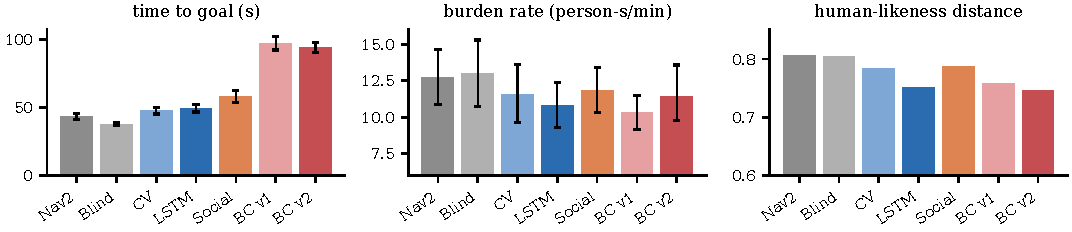
\includegraphics[width=\textwidth]{figs/results.pdf}
\caption{Time to goal and burden rate with 95\% bootstrap CIs, and human-likeness distance (lower is closer to the human driver).}
\label{fig:results}
\end{figure*}

\textbf{Prediction changes how the robot disturbs people, not how much.} With LSTM prediction, the robot pushed people off their paths 15\% less often per minute than Nav2 (paired difference $-1.9$ person-s/min, 95\% CI $[-3.3, -0.6]$). It also had the lowest human-likeness distance of all non-cloned set-ups. Its speed distribution moved towards the human's (Wasserstein 0.44 versus 0.66 for Nav2), and so did its speed towards nearby people (0.12 versus 0.23). However, it took 14\% longer to reach the goal, so total burden was the same as Nav2's (CI of the difference $[-1.5, +1.0]$ person-s). It also turned more (+18\% heading change per metre, CI $[+9, +27]$\%). Constant-velocity forecasts showed the same pattern, but weaker. Time within 0.5~m did not change; the 30\% reduction we had hypothesised for proximity was not met by any set-up.

\textbf{Slowing down costs people time.} The social yielding policy and both cloned drivers slowed the robot when people were near. This raised time within 0.5~m (Social $+0.9$~s, CI $[+0.5, +1.4]$), stop-starts (+42\%), time with TTC under 2~s (+53\%), and total burden (+32\%, CI $[+12, +53]$\%). People in TH\"OR-MAGNI walk about four times faster than the robot, so a robot that waits stays in their way for longer. Being near people was not, in itself, what produced burden.

\textbf{Ignoring people is not free, but nearly.} The blind control was fastest, made the fewest stop-starts, and had the lowest total burden. Its burden \emph{rate} was the highest, but only 2\% above Nav2's (CI includes zero). At this density, with people who step aside, Nav2's reactive avoidance changed little. This is the result we found most informative: it shows how easily a reactive crowd model can reward a robot that pushes through. Our model limits people to the effort real participants spent, which keeps the gap small but positive. With half-strength reactions, Nav2, LSTM and Social ranked the same way.

Fig.~\ref{fig:distributions} compares motion distributions. No set-up passed people at the human's clearance. The human driver's median passing clearance was \humPass~m, while all Nav2 variants passed most people within 1~m. The human operator also kept moving at a steady 0.2--0.3~m/s rather than switching between cruising and stopping. Prediction reduced Nav2's high-speed mode but did not reproduce either property.

\begin{figure*}[t]
\centering
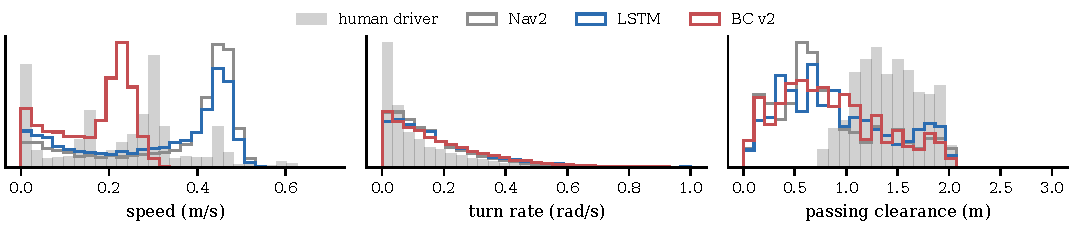
\includegraphics[width=\textwidth]{figs/distributions.pdf}
\caption{Motion distributions of three set-ups against the human-driven robot in TH\"OR-MAGNI (grey). Passing clearance is the closest distance to each person passed within 2~m.}
\label{fig:distributions}
\end{figure*}

\subsection{Cloning the human driver}
\label{sec:bc}
We trained LSTM policies to predict the operator's mean velocity over the next 0.8~s from 1.6~s of history. Inputs were the robot's own velocity, a subgoal (the operator's position 4~s later, in hindsight), and the six nearest people, all in a frame pointing at the subgoal. At run time, a node computes the same inputs, with the subgoal 1~m ahead on Nav2's plan, and turns the predicted speed into Nav2's speed limit.

Offline (Table~\ref{tab:bc}), the full model (BC-social) predicted the operator's velocity 8\% better than keeping the current velocity. However, it was no better than the same model without people (BC-blind), so people added nothing measurable. In closed loop, v1 (BC-social) drove at 0.16~m/s and failed to reach the goal in 22\% of runs. Its own past velocity let it copy itself: once slowed, it stayed slow. This is the copycat problem~\cite{wen2020copycat}. Removing that input (v2, BC-nocopy) halved the failures, but the robot still crawled at 0.17~m/s. The hindsight subgoal's distance encodes the operator's future progress, and therefore its speed. At run time the subgoal sits 1~m ahead, which in training meant an operator covering 1~m in 4~s (0.25~m/s), so the model drove slowly whatever the people did. This is a causal-confusion shortcut~\cite{dehaan2019causal}. Removing the subgoal too (BC-people) left a model that sees only people. It predicted speed worse than a constant and recognised only 10\% of the operator's yielding moments. The correlation between its predicted speed and the operator's speed was 0.06. In this dataset, the operator's speed was decided by things other than the nearby people, such as the task, the route and the operator's own habit, so it cannot be cloned from people alone. We did not run BC-people in closed loop.

\begin{table}[t]
\centering
\caption{Offline behaviour cloning on the held-out day. Vel.: velocity error (m/s). Speed: speed error when a person is within 2~m. Yield: share of moments with the operator under 0.1~m/s that the model predicts under 0.15~m/s.}
\label{tab:bc}
\begin{tabular}{llccc}
\toprule
Model & Inputs & Vel. & Speed & Yield (\%) \\
\midrule
Keep velocity & own velocity & \dvelKeep & \dspdKeep & \dyieldKeep \\
Goal pace & subgoal & \dvelGoal & \dspdGoal & \dyieldGoal \\
BC-blind & own vel., subgoal & \dvelBlind & \dspdBlind & \dyieldBlind \\
BC-social (v1) & all & \dvelSocial & \dspdSocial & \dyieldSocial \\
BC-nocopy (v2) & subgoal, people & \dvelNocopy & \dspdNocopy & \dyieldNocopy \\
BC-people & people & \dvelPeople & \dspdPeople & \dyieldPeople \\
\bottomrule
\end{tabular}
\end{table}

\section{Discussion and Limitations}
Our results support a narrow claim: a learned pedestrian predictor, added to an unmodified Nav2 stack, makes the robot disturb people less per minute and move more like a human driver. It does not reduce total disturbance or proximity, because the robot becomes slower. Methods that make the robot hesitate, whether hand-written or cloned, made things worse for people, which agrees with the freezing-robot argument~\cite{trautman2010unfreezing}. The human operator's advantage was keeping a wide berth while moving steadily. A planner cost that rewards clearance at constant speed, rather than a speed limit near people, is the natural next step.

The study has clear limits. The predictor and the governor receive ground-truth people positions, while Nav2's obstacle layers use the lidar. People in simulation are cylinders driven by a calibrated but simple reaction model, which cannot reproduce group behaviour or gaze. The human reference is one robot and a handful of operators in one lab, and the crowd is sparse (up to nine people). The navigation grid covers one held-out day (16 scenes). Finally, our burden metric assumes that being moved off one's recorded path is the main cost to a pedestrian; this is plausible but untested with real participants.

\section{Conclusion and Future Work}
Learning from a dataset that contains both pedestrians and a human-driven robot let us train a predictor, calibrate a reactive crowd, and define a human reference for robot motion. With these, learned prediction in Nav2 lowered the rate at which the robot disturbed people and brought its motion closer to the human driver's, while behaviours that slowed the robot added disturbance. The cloned driver failed for reasons that are well known in imitation learning, and we found that the operator's speed in TH\"OR-MAGNI does not depend on the people around it.

The next step is a driver dataset in which human operators react to crowds. SCAND~\cite{karnan2022scand} offers hours of teleoperated robots in public spaces, and MuSoHu~\cite{nguyen2023musohu} records humans navigating crowds with robot-like sensors. Both could supply a human reference and a policy whose speed and steering depend on people. We could not download SCAND during this work, and MuSoHu remains to be integrated. We also plan to learn a clearance-aware cost for the MPPI controller in place of a speed limit, and to validate the burden metric with real participants.

\section*{Code and Data}
Code, Nav2 configurations, trained weights, metrics for all episodes, rosbags and videos are available at \url{https://github.com/filmonnezif/social-nav-ros2}.

\bibliographystyle{IEEEtran}
\bibliography{refs}

\end{document}
